\subsection{Background}  
Many people always worry about what to wear tomorrow and waste a lot of time trying to find the cloth they want. Moreover, with the improvement of living standards, people pay more attention to how to dress better and how to choose a satisfying outfit according to different needs. To solve these problems, our group came up with an amazing solution —— An Intelligent System for Wardrobe! 

\subsection{Solution}
To address the problem stated above, we decided to build an intelligent system for the wardrobe. Whenever a user got a new cloth, he/she can wear the cloth and show the cloth to wardrobe. The wardrobe will take a photo of the cloth and label the cloth (labels could be “jeans”, “collared”, “woolen”, “red”, etc.). Moreover, the system will automatically allocate a coat hang for the new cloth. This is achieved by attaching a “Node MCU chip” with LED and button to the coat hang. This chip can exchange info with the remote server through Wifi connection. When the system finds a suitable coat hang, it will send a massage to light up that hang so that user can hang the cloth onto that. Then user will push the button to turn off the LED and notify the remote server that the new cloth has been successfully collected into the wardrobe. Every day when the user wakes up, he/she can ask the wardrobe to recommend what he/she should wear (the decision will be based on criteria like the weather, the place user want to go to, the color matched degree etc.) After the user become satisfied with what he/she will wear today. The wardrobe will use some method (e.g., LED light) to tell the user where the desired cloth is.

\subsection{Physical Design}

\begin{figure}[h]
   \centering
   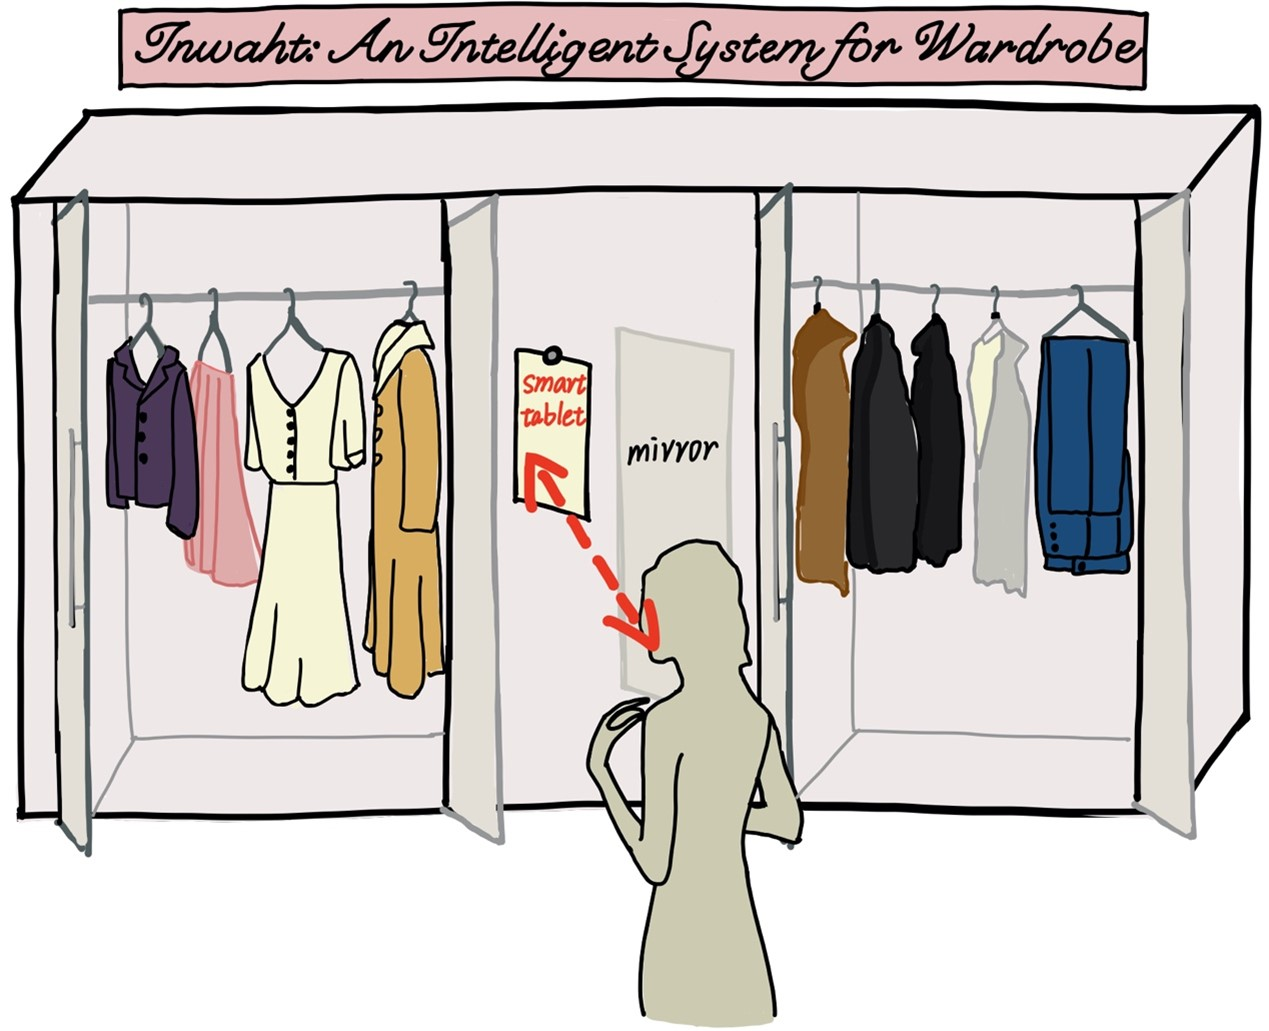
\includegraphics[width=8cm,height=6cm]{graph/physical design.jpg}
   \caption{physical design}
   \end{figure}

\subsection{High-level Requirements List}
\begin{itemize}
   \item[$\bullet$] Must recognize the feature of the cloth put in with an acceptable accuracy.
   \item[$\bullet$] Must have a usable recommendation function that give some valuable suggestion.
   \item[$\bullet$] Must have a user-friendly interface.
   \item[$\bullet$] Must let the user easily and quickly find where the chosen clothes are.
   \end{itemize}


